\documentclass[aps,pre,amsmath,amssymb,floatfix,onecolumn,notitlepage,10pt]{revtex4-1}
\usepackage{graphicx,isomath,bm}
\usepackage[colorlinks=true,linkcolor=blue,citecolor=blue,urlcolor=blue,pdfborderstyle={/S/U/W 1}]{hyperref}

\begin{document}

\title{On the glassy dynamics and the volcano transition of frustrated oscillators}
\date{\today}

\maketitle
%\tableofcontents

\section{Introduction}
Ottino and Strogatz recently published work \cite{strogatz} revisiting a longstanding problem in the theory of coupled oscillators. 
They propose a model of $N$ coupled oscillators with frustration,
\begin{equation}
\label{ode}
\dot{\theta}_j = \omega_j +J\sum_{k=1}^N A_{jk}\sin\left(\theta_k-\theta_j\right),
\end{equation}
with frequencies $\omega_j$ sampled from a Lorentzian distribution, $J$ a variable coupling constant, and $A$ an adjacency matrix defined by elements
\begin{equation}
\label{adjacency}
A_{jk} = \sum_{m=1}^{K}(-1)^m u_m^{(j)}u_m^{(k)}/N.
\end{equation}
Here, $u_m^{(j)}$ are random vectors with each element independent and equal to $\pm 1$ with equal probability. Since the signs of the adjacency matrix elements are random, the coupling is both attractive and repulsive,  leading to frustration. 

The adjacency matrix is formed by $K$ linearly independent (since each $u_m$ is random) rank-one updates, and so the rank of the adjacency matrix is $K$. For even $K$, the diagonal of $A_{ij}$ is also guaranteed to vanish. Ottino and Strogatz noted an interesting volcano transition for low-rank ($K\ll \log_2 N$) systems. In this case for $N\gg 1$,  they show that the incoherent state is unstable for $J>2$. For such parameters, clusters emerge,  and a low-dimensional Ott-Antonsen reduction suggests that the relaxation to this clustered state will be exponential. They numerically observe this exponential relaxation in the Kuramoto order parameter $r$ given by
\begin{equation}
\label{kuramoto}
re^{\Theta} = \frac{1}{N}\sum_{j=1}^N e^{i\theta_j}.
\end{equation}

They note that for large $K$, on the other hand, the Ott-Antonsen theory gives a high-dimensional system and the relaxation appears to be algebraic. However, the numerical simulations were limited and the evidence is not entirely clear. The main motivation comes from Daido's model for glassy dynamics in frustrated networks of coupled oscillators \cite{daido}. For $K=N\gg 1$, the adjacency matrix is well approximated by random matrix elements which are normally distributed (by the central limit theorem), which Daido studied previously.   Daido's relation to glassy dynamics was apparently contentious, and Ottino and Strogatz seemed to hope that their variable-rank model could shine a light on the question. However, the problem remains open.

Our main goal here is to apply data-driven methods to shine a light on the high-dimensional glassy dynamics in the large $K$ and large $N$ limit. One possibility we have considered is PCA or DMD analyses to try to infer the intrinsic dimensionality.  Another approach is to use SINDy on the dynamics of the order parameter to distinguish between the exponential and algebraic relaxation.  In the course of these studies, we have implemented efficient numerical integration on the GPU in order to observe the scaling for large $N$ and $K$ \cite{github}. Our efficient simulations are capable of exploring systems as large as $N=10^6$,  which is three orders of magnitude larger than those considered by Ottino and Strogatz. 

In exploring these larger systems, we have also noted subtlety in the glassy decay that could not have be recognized for the previously considered cases with $N<10^4$. In particular, we find that the decay only appears algebraic after an initial period of exponential decay. This onset period increases with increasing $N$.The balance between the scaling of the noise floor and the onset period with increasing $N$ is pertinent for the large $N$ limit.

\section{Analytical considerations}
Starting from a state of identical phases $\theta_i=0$, the system is expected to relax to the incoherent state for large $N$ and $K$ for which there is no clustering and the oscillator phases are uniformly random and indepdent. We can analytically predict the finite-$N$ scaling of the order parameter for this incoherent state. In this case,  the real and imaginary components of the complex order parameter will be sums of $N$ independent random variables (sampled by taking the cosine and sign of a uniform distribution). For large $N$, by the central limit theorem, these sums will converge to two independent normal distributions each with variance $1/2N$. The magnitude of the order parameter will then be distributed as a Rayleigh distribution with $\sigma=(2N)^{-1/2}$, and the mean magnitude of the order parameter is then 
\begin{equation}
r_{\mathrm{incoherent}}=\sqrt{\pi/4N}.  \label{incoherent}
\end{equation}
This is the ``noise floor'' observed in numerical simulations.

\section{Numerical considerations}
Ottino and Strogatz  used a fixed timestep $dt=0.01$ with a 4th-order Runge-Kutta method on a CPU.  We implement instead an adaptive time-stepping Dormand-Prince with a 5/4 embedding Runge-Kutta method on the GPU (the same method used by the ode45 in Matlab and the Python scipy method solve\_ivp).  The trajectory is sampled at the $dt=0.01$ timesteps using a ``free'' fourth-order polynomial interpolation. We reproduce both the low $K=2$ clustered states and the apparent high-$K$ algebraic decay to incoherence for $N=5000$ oscillators in Fig.~\ref{fig1}(a).

\begin{figure}[hbt]
\includegraphics[width=0.75\columnwidth]{fig1}
\caption{Volcano clusters for small $K$ and slow decay to incoherence for large $K$ for Lorenztian distributed frequencies with $J=2$ (a) and normal distributed frequencies with $J=1.75$ (b), with $N=5000$.  The noise floor from Eq.~\eqref{incoherent} is shown by the dashed black line.  Order parameters are averaged over $750$ simulations. \label{fig1}}
\end{figure}


Our first observation is that the fixed time step used by Ottino and Strogatz is not sufficiently small to guarantee an accurate solution for the problem with Lorentzian distributed frequencies, even for the small systems with $N=5000$ presented.  To control the error well, the timestep should be smaller than $O(T_m)$ where $T_m=2\pi/\omega_M$ is the natural period of the fastest oscillator since otherwise, the contributions to Eq.~\eqref{ode} will oscillate many times between time steps.  If the frequencies are distributed with a probability density $f(\omega)$, it can be shown that the distribution for the maximum frequency of $N$ samples is $Nf(\omega)F(\omega)^{N-1}$, where $F$ is the cumulative probability distribution, i.e. $F'(\omega)=f(\omega)$. So the expected maximum frequency is $\omega_M = \int N\omega f(\omega)F(\omega)^{N-1} d\omega$. For the standard Lorenzian distribution, this gives $\omega_M \sim 1.6475 N$ asymptotically for large $N$, leading to $T_m=0.0076$ for $N=5000$.  Indeed, our adaptive time step uses $dt\approx0.0015$ for $K=N=5000$. This scaling poses a significant challenge to increasing $N$ with Lorentzian-distributed natural frequencies. On the other hand, as shown in Fig.~\ref{fig1}(b), we observe a similar volcano transition for normally distributed natural frequencies in the small $K$ case, although the analytical Ott-Anstonsen predictions are not applicable and we find that the critical coupling $J_c$ is smaller than the value of $2$ in the Lorentzian case.   For the normal distribution, we find a much slower growth with $\omega_M < \log N$ (I'm sure some asymptotics can be done here as well...).   Thus, we opt to use normally distributed natural frequencies instead. In the normally distributed case, the adaptive time step does not become prohibitively small even for $N$ and $K$ up to $10^6$.

A second consideration for large $N$ and $K$ is the memory required to store the adjacency matrix. This requires at least $N\times K$ bits to store the $u_m(j)=\pm 1$ values, and, more simply, $N^2 \times 8$ bytes to store each floating point in the adjacency matrix.  Modern graphics cards typically have less than 20 GB of memory available, so this would constrain $N=K\lesssim 5\times 10^4$ if we store the entire adjacency matrix during the computation.  However, the numerical integration routine itself requires only $O(N)$ bytes of memory.  By careful use of the counter-based Philox64 random number generator, we can efficiently regenerate the numbers at an arbitrary position of a fixed random sequence without storing the entire sequence.  Thus, we can recalculate the adjacency elements in each CUDA kernel call only when required, and keep the memory requirements down to $O(N)$. Our limitation is then only the time required to integrate the system. In this way, it takes less than ten seconds to integrate $K=N=10^4$ oscillators and about two days to integrate $K=N=10^6$ oscillators with normally distributed natural frequencies. (Compare this with scipy integration on a CPU, which takes about two minutes for the $K=N=10^4$ case).

\section{SINDy fits}
We first contrast SINDy fits for $N=5000$ and $K=2$ or $K=N$. We average the order parameter $r$ over $750$ simulations with differing random seeds, and restrict the time interval to the period in which $5/\sqrt{N}<r<0.5$.  We use a polynomial library with terms up to order 5, and increase the threshold to eliminate as many terms as possible while achieving good fits. For $K=2$, SINDy discovers a model
\begin{equation}
\dot{r}_{\mathrm{pred}} = -2.258 r + 2.238 r^2,\label{sindy1}
\end{equation}
with the leading order linear term giving rise to the expected exponential decay. For $K=N$, we find a model
\begin{equation}
\dot{r}_{\mathrm{pred}} = -10.449 r^2 + 26.487 r^3 + -22.338 r^4.\label{sindy2}
\end{equation}
Interestingly,  the linear term is eliminated, and the leading order decay is expected to be algebraic. For both fits, the R2 score is greater than 0.99, and the comparison between the predicted $\dot{r}_{\mathrm{pred}}$ and the actual value $\dot{r}$ is shown in Fig.~\ref{fig2}.
\begin{figure}[hbt]
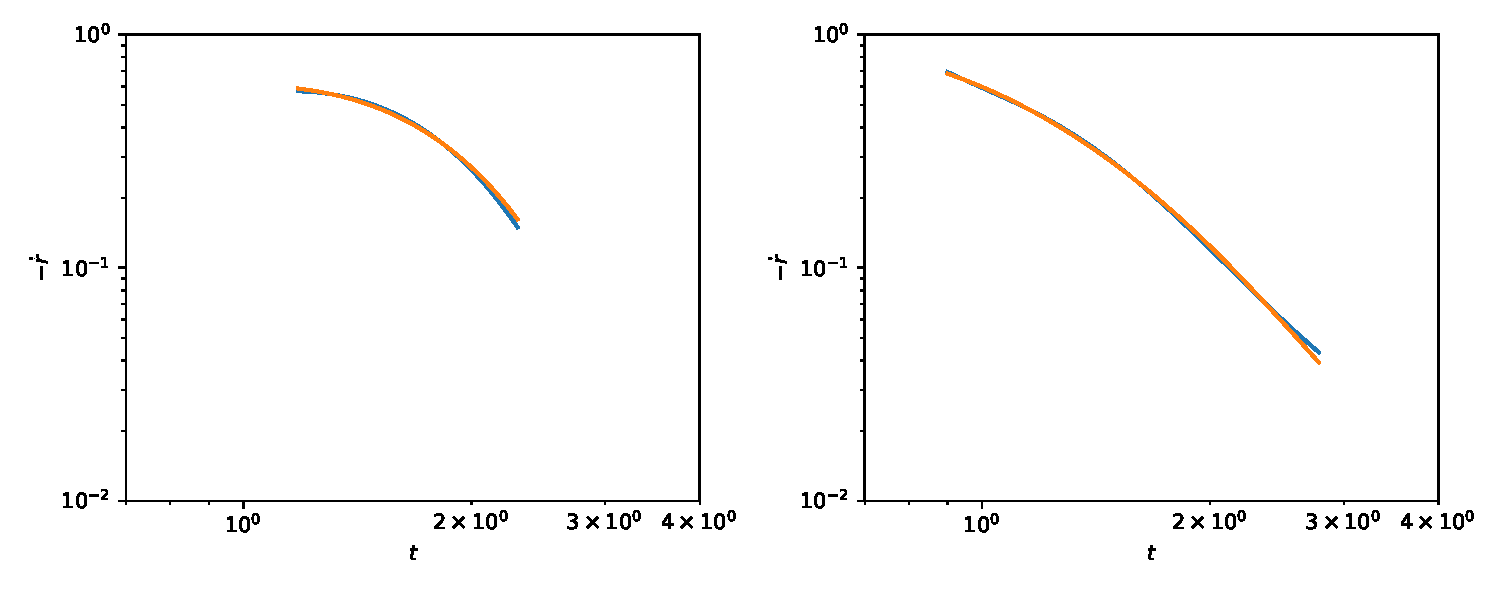
\includegraphics[width=0.75\columnwidth]{fig2}
\caption{SINDy predictions (orange lines) and actual time derivatives (blue lines) for the model in Eq.~\eqref{sindy1} with $K=2$ (a) and the model in Eq.~\eqref{sindy2} with $K=N=5000$ (b). \label{fig2}}
\end{figure}

\section{Large $N$ scaling}
Next, we consider the transition between the exponential and algebraic decay as $K$ and $N$ increase. Figure \ref{fig3} shows ours results for cases with $N\in(10^4, 2\times 10^4, 10^5,2\times10^5)$. We see that for intermediate $K/N$, there is a change from exponential to algebraic decay around $t=5$, with the time of onset of the transition increasing modestly with increasing $N$.  The rate of the algebraic decay decreases with increasing $N$, because the difference between the $O(N^{-1/2})$ noise floor in Eq.~\eqref{incoherent} and the values of $r$ at the transition time become increasingly small. Thus, the purported algebraic decay appears to be confined to an increasingly short period as $N$ increases, but the rate of decay is also increasingly slow. The limiting behavior as $N\to\infty$ is still unclear, but the simulations suggest a more complex asymptotics than previously suggested. (We may want to consider fixed $K=c\log(N)$ to try to fix the time of the onset of the transition.)
\begin{figure}[hbt]
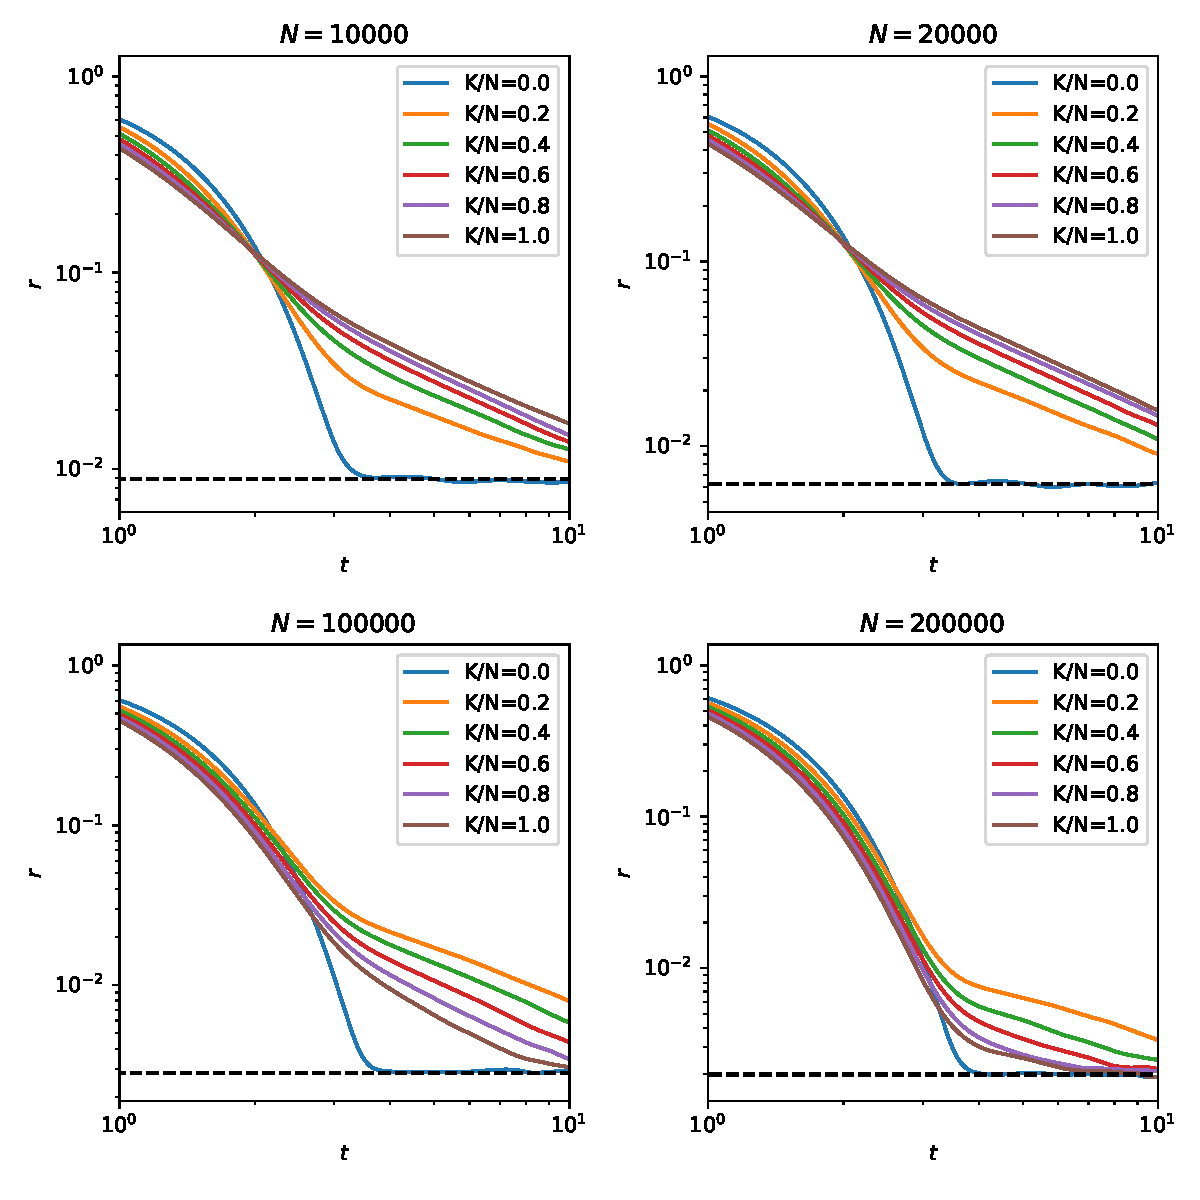
\includegraphics[width=0.75\columnwidth]{orders2.pdf}
\caption{Order parameter averaged over $500$ simulations vs time for various values of $N$ and $K$. \label{fig3}}
\end{figure}
\pagebreak

\begin{thebibliography}{99}
\bibitem{strogatz}Ottino-L\"{o}ffler, Bertrand, and Steven H. Strogatz. "Volcano transition in a solvable model of frustrated oscillators." Physical review letters 120, no. 26 (2018): 264102.
\bibitem{daido}Daido, Hiroaki. "Quasientrainment and slow relaxation in a population of oscillators with random and frustrated interactions." Physical review letters 68, no. 7 (1992): 1073.
\bibitem{github}See our github repository for source code and data: \url{https://github.com/znicolaou/kuramoto}.
\end{thebibliography}
\end{document}
